\documentclass[final-report]{report-template}

\usepackage{graphicx}
\usepackage{amsmath}
\usepackage{tikz}
\usetikzlibrary{arrows.meta, positioning, shapes.geometric}

\graphicspath{{./figures/}}

\university{Imperial College London}
\department{Department of Earth Science and Engineering}
\course{MSc in Applied Computational Science and Engineering}
\title{Current Content Discovery for Business Module Teaching}
\author{Guanyuming He}
\email{guanyuming.he24@imperial.ac.uk}
\githubusername{esemsc-gh124}
\supervisors{Sean O'Grady\\
             Rhodri Nelson}
\repository{https://github.com/ese-ada-lovelace-2024/irp-gh124}

\newcommand\casemethod{case method}
% allow breaking in long texttt words.
\newcommand\ttb{\discretionary{}{}{}}

\begin{document}

\maketitlepage  

\section*{Acknowledgements}
I would like to thank Sean for his constant meetings with me, providing user
feedback as a business school teacher, helping my project evolve.

I would like to thank Rhodri for his technical expertise that could hint me
with insights when I was stuck, without directly pointing out the direction.

Finally, I would like to thank Marijan for tirelessly answering my questions
about details of this IRP.

\subsection*{AI Acknowledgement Statement}
I have used two LLM tools to help with programming, each of which has
individual use cases:
\begin{enumerate}
	\item ChatGPT 4 and 5 (5 was released during the project, and OpenAI forced
		the switch. I did not intentionally switch to it for any reason.)
		\textbf{Publisher}: OpenAI. \textbf{URL}: \url{https://chatgpt.com/}.
		\textbf{Usage}: \emph{Help me diagonose errors like C++ compilation or
		linkage errors; suggest libraries alternatives when one didn't work;
	help me learn to use a third-party library or Python module fast.}
	\item Claude AI. \textbf{Publisher}: Anthropic. \textbf{URL}:
		\url{https://claude.ai/}.  \textbf{Usage}: \emph{Help me generate very
			(logically) simple code that would be tedious to write to hand.
			Three cases in my project: 1. tedious GUI elements creation (not
			all GUI elements; some special UI elements are manually written) 2.
			tedious logging (I adjusted the logging sentences).  3. tedious
			unit test cases (not all cases. Some cases are special and I
			manually wrote them). I also review and adjust generated code.}
\end{enumerate}

I confirm that all submitted works are my own, despite the assistance from those
LLM tools.

\section*{Abstract}
Business school teaching using the well-known \casemethod\ requires a
substantial amount of information about latest business events to keep the
course relevant.  Digital technologies like web search engines and LLMs can
offer substantial assistance to this process. However, several challenges
remain: 1) search engines struggle to process unstructured search queries. 2)
while LLMs excel in understanding unstructured input, they have problems in
ensure the accuracy and timelyness of retrieved information. 3) these tools
still require manual invocation. In this project, I aim to address these
challenges by a software system that compensates search engines and LLMs with
each other, while also supporting automatic execution of the whole process and
the delivery of the results to users, requiring minimal user configuration.

\textbf{Keywords:} information retrieval, LLM, search
engines, \casemethod, Business school

\section{Introduction}
\subsection{Project background} \label{sec.proj.bg}
Since the emergence of the first Business schools in the late 19th century
\cite{first.bis.school.1, first.bis.school.2}, several distinct pedagogical
teaching strategies have been invented.  First institutionalized at Harvard
Business School \cite{case.method.origin.1, case.method.origin.2} in the early
20th century, a method about teaching students with real world business cases
(will be called \emph{\casemethod} in the rest of the thesis) has been found
more effective and engaging \cite{case.method.support.1, case.method.support.2,
case.method.support.3} than many traditional, for example, big lecture based,
teaching methods. Thus, it obtained wide adoption across the world
\cite{case.method.adoption.1, case.method.adoption.2}.

Despite its aforementioned adoption and performance in business school
teaching, the \casemethod\ faces a significant constraint: the availability and
collection of timely and relevant case material \cite{case.method.limit.1,
case.method.limit.3}. In particular, Christensen identifies in his classical
article that instructors have to conduct ``extensive preparation''
\cite{case.method.limit.2} for it. Another reason is the ever-evolving business
world and the necessity of the latest information: Clark argues that learned
skill will lose value quickly in five years, and then it is critical for
students to be up to date to remain relevant in the business world
\cite{case.method.limit.4}; McFarlane emphasises the importance of updated
cases, as otherwise students could be disengaged or discouraged
\cite{case.method.limit.5}.

\subsection{Past advancements in information retrieval} 
\label{sec.info.ret.history}
The thesis summarizes the challenges in information retrieval into two general
problems: 
\subsubsection{Problem (1): collect/gather information}
During the past two centuries, several key developments have profoundly
expanded one's capacity to gather information about the world. In
the early 19th century, the transmission of information was still traditional
--- carried by person on paper or simply remembered. The invention of
telegraph in the 1840s by Morse et al.\ \cite{history.telegraph.1,
history.telegraph.2}, notably with Morse's first telegraph message,
``\emph{What hath God wrought?}'' in 1844 \cite{first.telegraph.msg}, marked a
paradigm shift. This technological innovation was considerably improved by
Bell's telephone in 1876 \cite{history.telephone.1, history.telephone.2},
enabling communication directly by human voice, instead of encoded Morse code.

Wired communication is critically constrained by geographical features (where
the wires were laid). Around the late 19th century, Marconi's experiments with
wireless telegraphy \cite{history.wireless.1} and the first successful
transatlantic signal in 1901 \cite{history.first.atlantic.broadcast} introduced
wireless communication, eventually accumulating into the world's first voice
broadcast by radio in 1906 \cite{first.voice.broadcast}. These milestones
collectively redefined the temporal and spatial boundaries of information
gathering.

Parallel to improving the weaknesses of wireless communication
\cite{wireless.weakness.1, wireless.weakness.2, wireless.weakness.3},
reseachers also worked on a theory of information.
Hartley observed a logritham pattern of information capacity
\cite{hartley.log.information} and then Shannon expanded on it to first define
\emph{bits} and \emph{entropy}, giving a formal mathematical theory of
information \cite{shannon.theory.communication} in 1948. Meanwhile,
engineers were experimenting with alternative modulation techniques, notably
frequency modulation (FM), and the concepts were formalized in the 1930s
\cite{history.modulation}. 

\subsubsection{Problem (2): identify/find desired information from collection}
Although solutions to problem (1) had enormously improved during these times,
substantial progress in problem (2) would have to wait until digital computers
were invented in the 1940s \cite{eniac.story}, which were made to repeat
tedious operations fast. Actually, the term \emph{information retrieval (IR)} was
not there until Mooers coined it in 1950 \cite{mooers.info.ret.term}.  The
nature of information reveals two subproblems of problem (2): (2.1) how to
process (extract useful information from) potentially unstructured data. (2.2)
how to related human queries to the content a user actually wants.

According to Griffiths and King, early IR systems (in the USA) were mainly
transferring human computing activity (bookkeeping in a library or database)
into digital forms, by various sorting, indexing, and searching algorithms
\cite{early.info.systems}. The form slowly went from ``offline, batch''
computing to ``online, real-time'' computing, and finally became ``distributed,
networked, and mass computing'', thanks to the Internet and various of its
applications \cite{early.info.systems, history.internet}. Then commercial
search engines emerged in the 1990s, opearting on the scale of the whole
Internet \cite{history.search.engines, history.internet.search.engines}.

The aforementioned sorting, searching, and indexing algorithms were partial
solutions to problem (2.1) and (2.2), with fundamental designs like inverted
index \cite[chap.~2]{intro.info.ret}, \cite[sect.~2]{inverted.files.search},
boolean search \cite[chap.~1]{intro.info.ret}, and various clever ideas such as
spelling correction (stemming) \cite[chap.~3.3]{intro.info.ret}, positional
indexing \cite[sect.~3]{inverted.files.search}. Because the database can be
extremely large, specific index construction \cite[chap.~4]{intro.info.ret},
\cite[sect.~5]{inverted.files.search} compression
\cite[chap.~5]{intro.info.ret} algorithms have appeared. Also, people saw ample
opportunity to explore distributed computing, with the most notable model
probably being MapReduce \cite{mapreduce}.

Nevertheless, these inventions were still mostly doing textual processing, and
machines struggled to ``understand'' information. Thus, advanced and complex
search queries are often needed to achieve desired performance
\cite{advanced.search.necessity.1, advanced.search.necessity.2}. The research
on making computers understand natural language (NLP), images and visuals
(computer vision), etc.\ were consequently and gradually being integrated into
search engines, since 2000, notably with Google's Panda, Penguin, and
Hummingbird algorithms that aim to understand web content better to rank them
in searches \cite{google.new.algos}.

One major breakthrough in NLP is Vaswani et al.'s transformer \cite{transformer}. 
Building upon it, OpenAI created generative pre-trained transformers (GPTs)
trained on massive amount of data \cite{gpt1}, which, after a few iterations,
evolved into a chatbot facing the general public, ChatGPT, and it was perhaps
then when LLMs started to recieve massive amount of public attention. Here, LLM
stands for large language model, language models that are \emph{large} in
trained data and parameters.

Although public attention is not the same as academic importance, LLMs
have undoubtedly entered and transformed many areas, including daily life,
business and the industry, and research \cite{llm.impact.1}. One strong appeal
of LLMs is that they could process unstructured natural language input and generate
natural language output in return with remarkable resemblence to what a human
would say \cite{llm.power.1, llm.power.2}. However, because of the inherent
limit of neural networks, some raise concerns about their formal reasoning
capabilities \cite{llm.limit.1, llm.limit.2, llm.limit.3}. Indeed,
hallucination \cite{llm.hallucination.1, llm.hallucination.2} and other forms
of distortion of facts, is a big problem of LLMs.

Despite the drawbacks of LLMs, they are currently the most successful tool in
NLP, and naturally various attempts have been made to integrate LLMs with search
engines \cite{llm.meet.search.1, llm.meet.search.2, llm.meet.search.3}.
Specifically, Xiong et al.\ proposes to categorize them into ``LLM4Search'' and
``Search4LLM'', where ``A4B'' means using A to improve B
\cite{llm.meet.search.1}. Here is where my thesis will build upon.  Now, with
the help with LLMs that can easily process frivolous natural language input, I
plan to integrate them together to boost an individual's information retrieval
further, especially in the area of business school teaching content discovery.

\subsection{Contemporary related work} \label{sec.related.work}
\subsubsection{Retrieval augmented generation}
During training, LLMs turn training data into their parameters (also
parametric-memory). Its immutability after training is a
weakness for information/knowledge based tasks, as information
cannot be easily added without retraining. RAG is a general approach to
fine-tune a trained model with non-parametric memory \cite{rag}. 

RAG was designed to enrich a trained LLM with a pre-trained retriever.
Addressing hallucination is its major concern. Because the retriever also
needs to be pre-trained, it cannot inherently solve the outdated training data
problem. In fact, their work's retriever, also a neural network, was trained on
a 2018 Wikipedia dump \cite[Section 3]{rag}.  These are the major differences
from my work.

\subsubsection{Other hybrid methods}
Beside RAG, numerous studies were conducted to augment pre-trained LLMs with
external knowledge \cite{hybrid.method.1, hybrid.method.2, hybrid.method.3,
hybrid.method.4, webgpt}.
Some worked on the retriever, some on how information is integrated into the
LLM, and some on both. Unlike my work, they focus on question-answering
tasks, and none of them had getting the latest information as a requirement.

Among them, Nakano et al.'s WebGPT is perhaps the closest to my work: their
retriever is a text-based web-browser \cite{webgpt}. Nevertheless, WebGPT was
designed to answer long-form questions, trained primarily to answer questions
from a specific dataset. Moreover, it used human feedback to improve quality.
These are the differences from my work.

\subsubsection{Search engine centric}
As the aforementioned studies work on improving LLMs, various works are also
committed to improve search engines. Some of them rewrite and improve search
queries with LLMs \cite{query.rewriting.1, query.rewriting.2}; some turn to
assist ranking of search results \cite{search.result.rerank.1,
search.result.rerank.1}. My work has both elements: in my project LLM will both
be used on search queries and on search result synthesis.

Furthermore, LLMs can potentially help document indexing with their excellent
NLP abilities in term extraction \cite{llm.term.extraction.1,
llm.term.extraction.2} and document filtering \cite{llm.indexing.filter},
although the first two cited work do not primarily consider search engine
applications. 

\subsection{Goals} \label{sec.intro.goals}
\begin{enumerate}
	\item By combining LLMs and search engines, compensate each other's
		weakeness in information retrieval.
		\begin{enumerate}
		\item The system shall improve search engines so that a user would only
			need to give a rough and vague natural language description of the
			target information to the system.
		\item The system shall improve LLMs on result reliability and
			accuracy. If pure LLMs lack the two properties, then combination
			with deterministic search engines, using deterministic and accurate
			algorithms.
		\end{enumerate}
	\item Enhance the automation of the current general public information
		retrieval tools, e.g., Google search, ChatGPT, so that
		user would only need to occasionally configure the system for it to
		schedule running automatically.
	\item Specially tailor the system to business teaching related information,
		aiming to gather information from authentic and reliable sources.
	\item The system shall support up-to-date information retrieval. It should
		support restricting the date range of results.
	\item (Optional) The system could support user feedback and learning from
		it.
\end{enumerate}

\subsubsection{Not in the goals}
\begin{enumerate}
	\item Providing a method to rank business information. That is rather
		subjective.
	\item Design, build, and train a LLM. That is too much work.
\end{enumerate}

\section{Methods} 
\subsection{Design philosophy} \label{sec.design.philo}
The core of this project is a big software system designed to achieve the
goals. Considering the scale and complexity of the software system, its
development will greatly benefit from a clear design philosophy.

The design philosophy is a set of the following philosophical approaches
to develop the system. Approaches 1--3 are from MIT Software Construction
\cite{mit.software.construction}. Approach 4 is part of the Unix
philosophy \cite{unix.philosophy}.

\begin{enumerate}
	\item 
	\emph{Correct today and in the unknown future}: By developing the
	system using design concepts like abstract datatypes \cite{adt},
	immutability, and software testing, its current correctness is defended;
	by defensive programming (type safety, robust checks, etc.), its
	correctness is defended from my future mistakes and stupidity.
	\item 
	\emph{Easy to understand}: Via thorough documentation, static type hints,
	and again immutability, the code can communicate well with the future me
	who may need to fix bugs or extend the system.
	\item
	\emph{Ready for change}: The system should be designed to make extensions
	easy; it would not be ideal to discard and rewrite a lot of code for
	extensions. 
	\item
	\emph{Do one thing and do it well}: The system is composed of a collection
	of programs, each of which is designed to do one particular job, and all of
	which are designed to work together.
\end{enumerate}

\subsection{Architecture}
As clarified previously, the system is a collection of programs working
together. What threads them together is a pipeline, taking the user's
configuration as input to produce current information about the business topics
mentioned in the configuration as output. The workflow of the pipeline is:
\begin{enumerate}
	\item LLMs generate a list of search engine prompts based on the business topics
		in the configuration.
	\item The prompts are fed to search engines.	
	\item The search results are gathered and filtered. In particular, filter
		by date.	
	\item The processed results are synthesized by LLMs.
	\item The results are sent to the users via the configured ways.
	\item Optionally, the user gives feedback to the results. 
\end{enumerate}

The pipeline needs to retrieve current information from somewhere. Thus,
another big module of the system is a minimal web search engine that can index
business news websites for latest news. The purpose of this self-made search
engine is to provide explicit control of the indexed contents and to avoid
commerical limitations on the usage. See section \ref{sec.custom.search.engine}
for the complete discussion. Still, third-party search engines are also used to
improve result coverage.

Surrounding the pipeline and the search engine are the supporting programs
which handle automation, output delivery, and user-friendly (GUI) configuration
management. Table \ref{table.all.programs} lists all programs in the system and
their functionality. They are not full paths, to not overflow the table. The
C++ programs can be found in \texttt{src/\ttb CMakeLists.\ttb txt}; the Python
scripts can be found in \texttt{src/}.
\begin{table}[hbtp!]
\centering
\begin{tabular}{|p{4cm}|p{10cm}|}
	\hline
	\verb!indexer!, \verb!searcher!, \verb!updater! &
	Build a search engine database from scratch, search a database, and update a
	database by adding new entries from RSS and removing old ones,
	respectively. 
	\\ \hline
	\verb!rm_doc!, \verb!upd_doc! &
	Tools intended for the developer (me) to fine-tune the database by removing
	and updating specific documents in it, respectively.
	\\ \hline
	\verb!llm_pipeline.py! & The main pipeline program. 
	\\ \hline
	\verb!config_gui.py! & A user friendly GUI program to configure the system.
	\\ \hline
	\verb!search_combined.py! & Obtains the search result from my custom
	search engine as well as Google, filters them, and combines them.
	\\ \hline
	\verb!setup_schedules.py! & Schedule automatic executions for various
	programs in the system to make the system automatic.
	\\ \hline
	\verb!tests/*! & Unit tests	
	\\ \hline
	\verb!misc/*!, \texttt{doc\_\ttb dist} & Miscellaneous programs for
	analyzing the system in the results section.
	\\ \hline
\end{tabular}
\caption{All programs in the software system}
\label{tab.all.programs}
\end{table}

Figure~\ref{fig.arch.flow} demonstrates my architecture design and the workflow
of the system, where blue boxes form the pipeline, the yellow boxes are the
other supporting programs, and the red box with the dashed lines are optional.
\begin{figure}[htbp!]
\centering
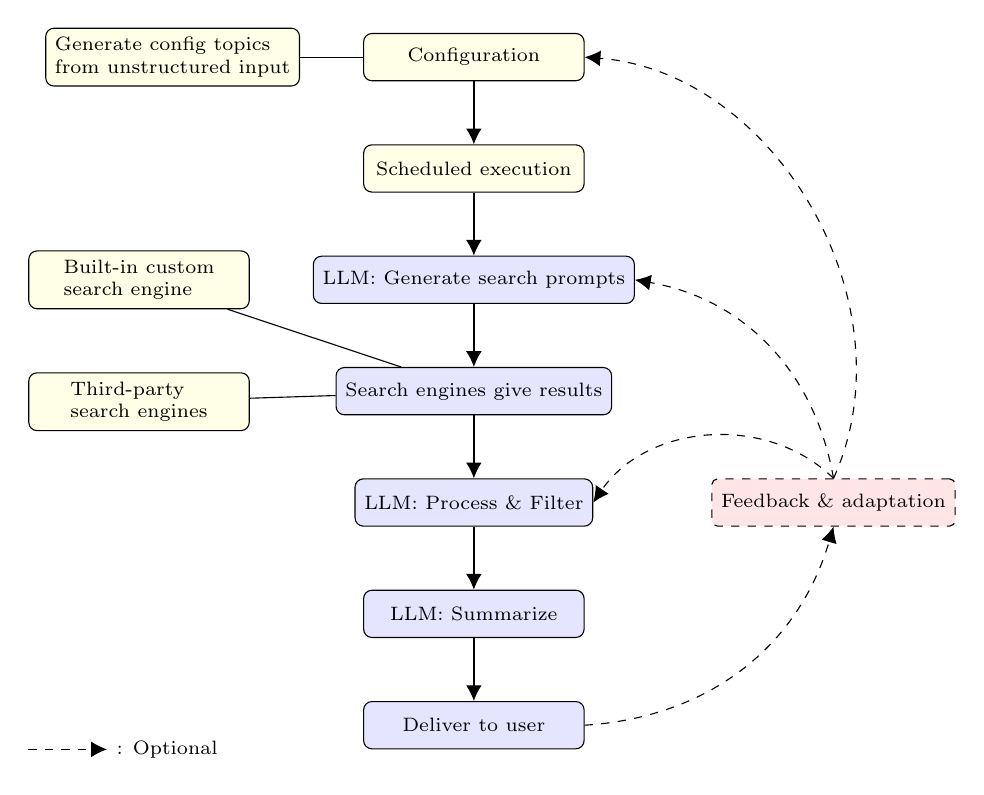
\begin{tikzpicture}[
	  node distance=0.8cm,
  every node/.style={font=\scriptsize},
  process/.style={draw, rounded corners=3pt, fill=blue!10, minimum width=2.8cm, minimum height=0.6cm, text centered},
  module/.style={draw, rounded corners=3pt, fill=yellow!10, minimum width=2.8cm, minimum height=0.6cm, text centered},
  feedback/.style={draw, dashed, fill=red!10, rounded corners=2pt, minimum width=2.6cm, minimum height=0.6cm},
  arrow/.style={-{Latex[width=2mm,length=2mm]}, line width=0.5pt},
  fb/.style={-{Latex[width=2mm,length=2mm]}, line width=0.4pt, dashed, bend right=35}
]

% Main vertical flow
\node[module] (config) {Configuration};
\node[module, below=of config] (scheduler) {Scheduled execution};
\node[process, below=of scheduler] (promptgen) {LLM: Generate search prompts};
\node[process, below=of promptgen] (search) {Search engines give results};
\node[process, below=of search] (processresults) {LLM: Process \& Filter};
\node[process, below=of processresults] (summarize) {LLM: Summarize};
\node[process, below=of summarize] (deliver) {Deliver to user};
\node[feedback, right=1.5cm of processresults] (feedback) {Feedback \& adaptation};

\node[module, left=of config, align=left] (genconfig) {Generate config topics\\from
	unstructured input};
\node[module, left=of promptgen, align=left] (builtinsearch) {Built-in custom\\search
	engine};
\node[module, below=of builtinsearch, align=left] (thirdsearch) {Third-party \\search
	engines};

% Links (supporting program involvement)
\draw (genconfig) -- (config);
\draw (builtinsearch) -- (search);
\draw (thirdsearch) -- (search);

% Arrows (main pipeline flow)
\draw[arrow] (config) -- (scheduler);
\draw[arrow] (scheduler) -- (promptgen);
\draw[arrow] (promptgen) -- (search);
\draw[arrow] (search) -- (processresults);
\draw[arrow] (processresults) -- (summarize);
\draw[arrow] (summarize) -- (deliver);

% Optional arrows
\draw[fb] (deliver.east) to (feedback.south);
\draw[fb] (feedback.north) to (promptgen.east);
\draw[fb] (feedback.north) to [bend right=50] (processresults.east);
\draw[fb] (feedback.north) to [bend right=55] (config.east);

% Legend
\draw[fb] (current bounding box.south west) -- +(1,0)
	node[right]{: Optional};
\end{tikzpicture}
\caption{Architecture and operational flow of the software system}
\label{fig.arch.flow}
\end{figure} 	

\subsubsection{Search engines} \label{sec.custom.search.engine}
The easiest way to integrate a web search engine is to use a commerical search
API, building upon the large database the commerical company provides.
However, this suffer from a few serious problems.
\begin{enumerate}
	\item 
	The free-tier APIs often have various ungenerous limits, e.g., number of
	queries, number of results returned, and filtering of search results.  For
	instance, see Google's \cite{search.api.limit.1}.
	\item
	The mechanism of the search engines is proprietory; I cannot control what
	they give. This is a big problem, because my goal is not about retrieving
	general information but specific information of business teaching value.
\end{enumerate}

Therefore, I plan to use my custom minimal search engine alongside commerical
search APIs. The custom search engine will address the two problems with
unlimited usage and specific information retrieval. To achieve the latter, I
configure the search engine to \emph{only} index business news websites.
Clearly, I will not have the resource to index most of the Internet and store
them, and this coverage weakness will be compensated by the use of commercial
search APIs.

\subsection{Implementation detail}
Following the design philosophy and architecture, here are the details of the
implementation.

\subsubsection{Configuration format} 
Most of the configuration have to be exact, e.g.,
\begin{enumerate}
	\item Scheduled time of the executions.
	\item A list of email addresses to deliver the results to.
	\item System prompts.
\end{enumerate}

The business topics in the configuration are used as input to the system.
Here, LLMs will be used to extract them from unstructured data, including both
user natural language input and images input\footnote{For all the configuration
entries, see \texttt{config.py}.}.

\subsubsection{LLM invocation}
Considering the heavy use of LLMs and the strict limitation of commercial LLM
APIs \cite{openai.api.limit, anthropic.api.limit}, the project will use local
LLMs powered by Ollama \cite{ollama}.

Ollama provides two main modes to communicate with LLM, \texttt{generate} and
\texttt{chat}; both access the Ollama local server at \url{localhost:11434} via
HTTP POST. Because the system is not interactive, only the \texttt{generate}
method is used.

Apparently, the system prompts are essential to our tasks. There is
generally no fixed algorithm to derive the best prompts given to LLMs, as
the results not only depend on many aspects including how the input is
given, but also probably are not deterministic, given that probalisitic
processes are widely used in deep neural networks and complex machine learning
models. Thus, the only way to obtain desirable prompts is to manually craft the
prompts and test them.

Initially, each stage invoking LLMs was one-shot (using only one invocation of
the LLM). Later tests revealed that this approach was extremely hard to tune
for all situations. Therefore, I turned to have a multi-stage invocation for
each step, enabling the LLM to focus on one specific task at one time.

The manual tests are done in two ways. The straight-forward way is to directly
change the prompts in my system, which is easy, thanks to the fact that I
put them in configuration. Still, this requires running a large part of the
system and is inefficient. Another approach involves OpenWebUI
\cite{open.webui}, a GUI tool that allows me to interact directly with the LLM
models via a web UI. Note that the models  there are in \texttt{chat} mode
instead of \texttt{generate} mode. Nevertheless, practice proved that prompts
good in chat mode is still useful in the generate mode.

The LLM models are selected prioritizing usability on personal computers. Thus,
the maximum number of parameters is limited. Among all the models Ollama offers
\cite{ollama.models}, I chose \texttt{llama3.1:8b} for its competitive ability
on text generation and summarization, proven by several academic studies and
benchmarks \cite{llama3.1.bench.1, llama3.1.bench.2, llama3.1.bench.3}.
Unfortunately, llama3.1:8b is text-only. When the user uses images to generate
business topics, as mentioned earlier, another model fine-tuned with llama3
instructs, \texttt{llava-llama3}, is used.

\subsubsection{Search engines}
My custom search engine is implemented in C++ with
\href{https://curl.se/libcurl/}{\ttfamily libcurl} for url handling,
\href{https://lexbor.com/}{\ttfamily lexbor} for HTML parsing, and
\href{https://xapian.org/docs/}{\ttfamily xapian} for database building and
searching. Also, \href{https://pugixml.org/}{\ttfamily pugixml},
\href{https://www.boost.org/}{\ttfamily boost.url, boost.test}, and
\href{https://github.com/amosnier/sha-2}{\ttfamily amosnier/sha2} are used as
support libraries. Finally, Python is linked to call Python functions inside
C++.

The custom search engine's algorithm is similar to the mainstream ones:
Starting from initial urls, scrap each. And for every url found in each, scrap
them too.  More precisely, the indexing of a webpage and the recursion into its
urls included are controlled by four predicate filters. Two are on URLs and two
are on the webpages. A webpage is indexed if both URL \& webpage index
predicates return true; each of its url is considered further if both URL \&
webpage recurse predicates return true. I separate the URL \& webpage
predicates because I can then delay scraping of a webpage only after its URL
passes the conditions.

When search prompts generated by LLMs are given, they will be fed to both my
custom search engine and Google's programmable search engine, with their
results combined and filtered.

\subsubsection{Task Schedulling}
The scheduled tasks are installed on the target operating system via
\href{https://en.wikipedia.org/wiki/Cron}{cron}, a task scheduler on Unix-like
systems. Before the tasks are actually installed, the installer script will
check if two jobs execute at the same time and abort the installation if they
do, to avoid parallel access to the custom search engine database.

\subsubsection{Report delivery} 
The results, finally summarized as a report, is sent to the users automatically
via email. Because the code is visible in the repository along with the login
credentials, I registered a burner Google account for email delivery. The
configuration records a list of destination email addresses, to each of which
the final results of running the pipeline will be sent from the burner account.
The protocol is SMTP + TLS to ensure that the email content is confidential.


\section{Results}
This section demonstrates the completed system.  Next, using the same inputs,
information retrieved by mainstream LLMs \& search engines are also displayed
for comparsion.

As a Business School teacher, Sean O'Grady provides me with a list (LIST 1) of
topics from his modules which will be used as inputs for demonstrating results.
\begin{enumerate}
	\item Vertical integration
	\item Diversification 
	\item Competitive advantage
	\item Foreign direct investment
\end{enumerate}

\subsection{Completed system}
\subsubsection{Configuration GUI}
The GUI used for end-users to configure the pipeline is implemented in Tkinter
\cite{tkinter}, a Python GUI interface. By the principles in section
\ref{sec.design.philo}, the configuration is divided into different separate
\texttt{Config\ttb Section}s, each of which is managed by a GUI class
inheriting from base class \texttt{Config\ttb Section\ttb Frame}\footnote{The
source is in \texttt{config\_\ttb gui.py}.}.

Figure~\ref{fig.config.gui} is a screenshot of the GUI.
\begin{figure}[hbtp!]
	\centering
	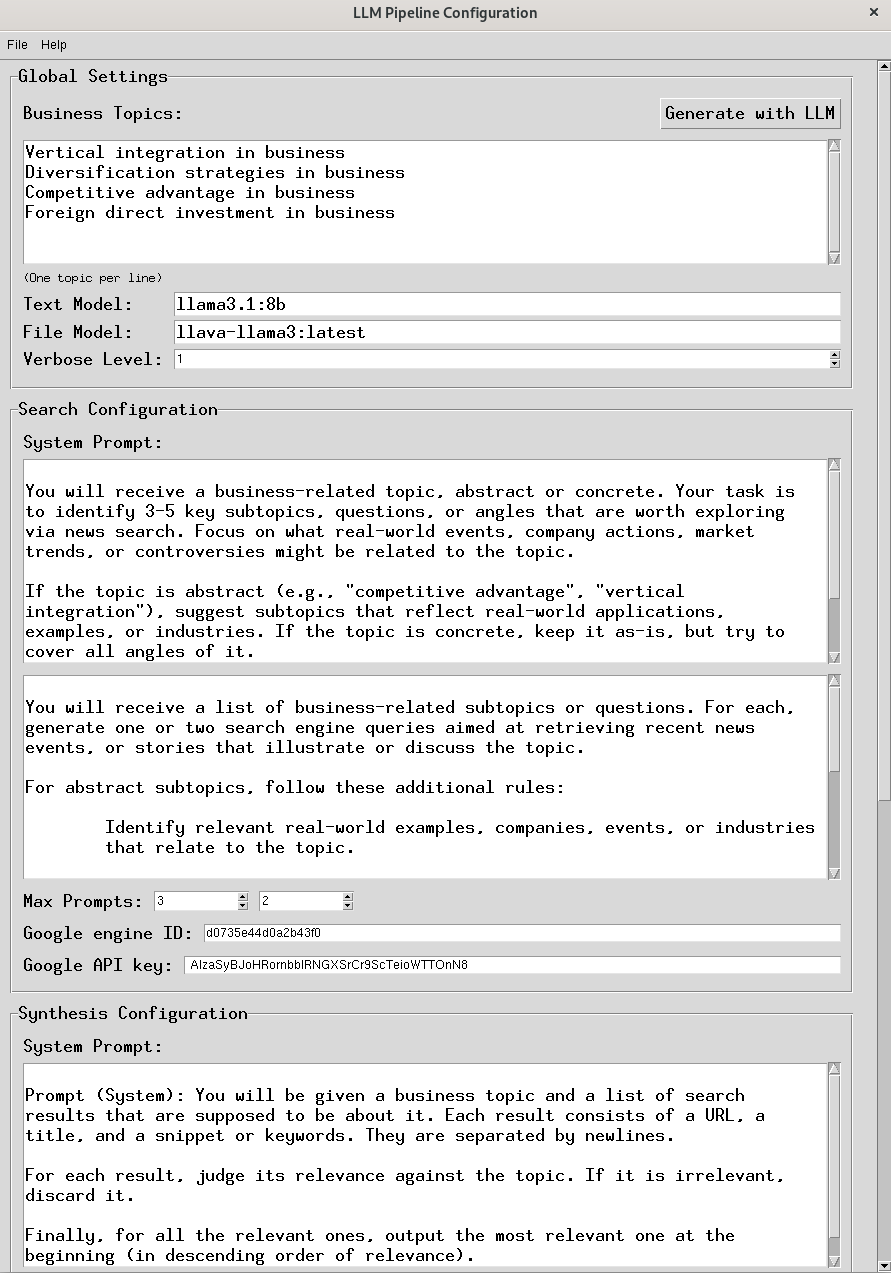
\includegraphics[height=.25\textheight]{res/gui.png}
	\caption{Configuration GUI}
	\label{fig.config.gui}
\end{figure}

\subsubsection{Custom search engine}
Recall that the main goal of developing this custom search engine is to
restrict information sources by explicit control over it.
Figure~\ref{fig.index.host.dist} displays\footnote{Produced by \texttt{src/\ttb
	misc/\ttb doc\_\ttb dist\_\ttb pie.py} and \texttt{src/\ttb search/\ttb
tools/\ttb doc\_\ttb dist.cpp}} the host distribution of all the indexed data
on my personal computer, as of 7 August. Unfortunately, because of the
volatility of the Internet content, the exact data is probably not
reproducible. Arguably, all domains from the database are reputable Business
news publishers.
\begin{figure}[hbtp!]
	\centering
	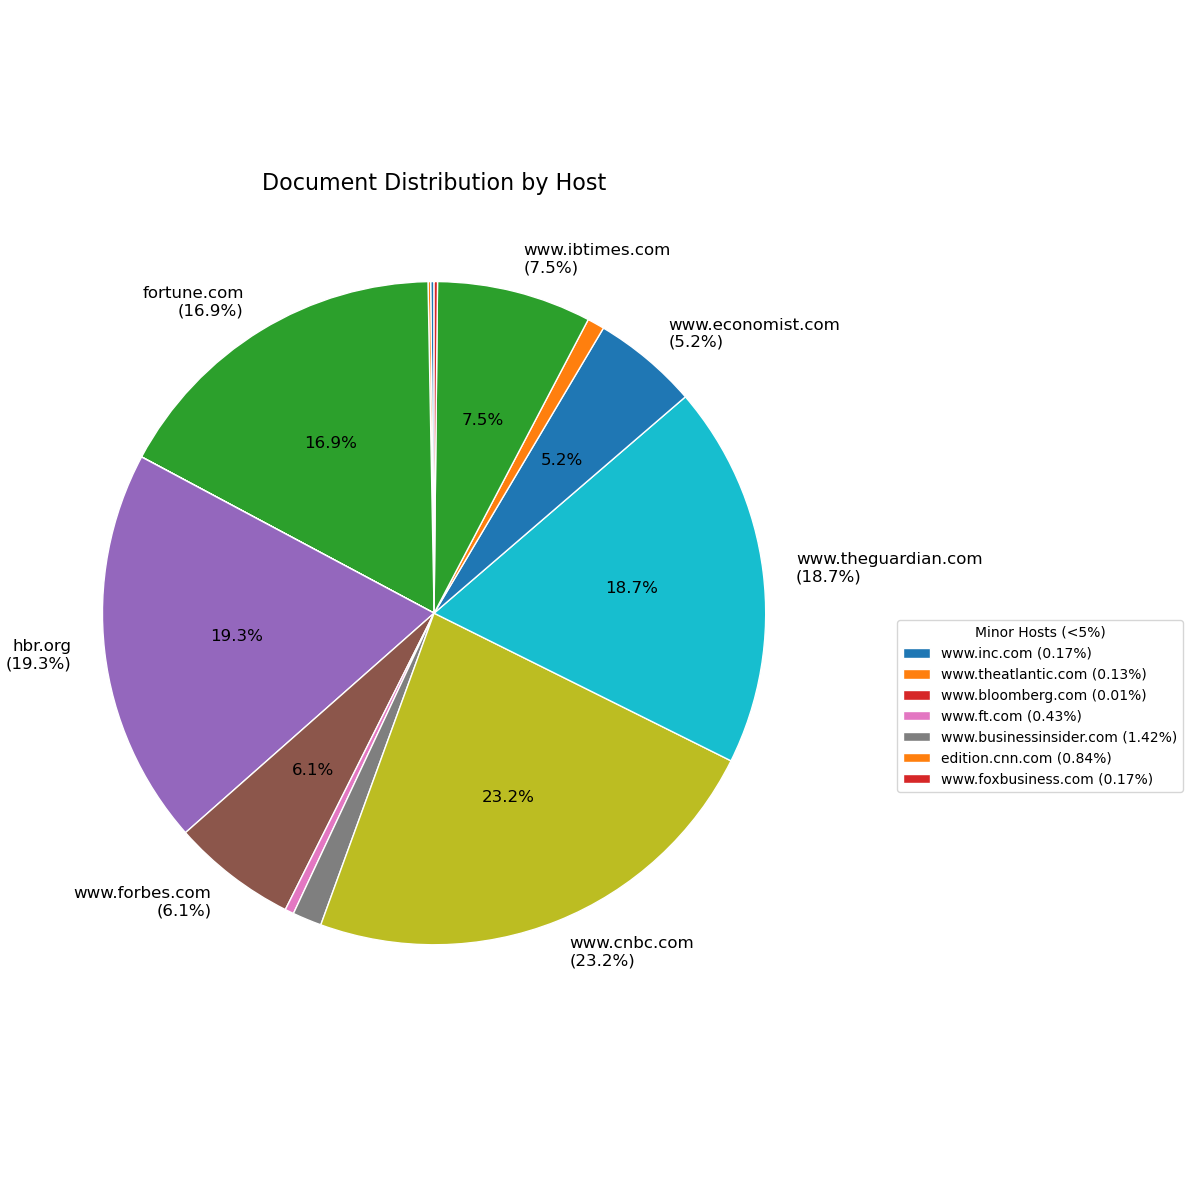
\includegraphics[height=.35\textheight]{res/doc_host_dist.png}
	\caption{Indexed document host distribution}
	\label{fig.index.host.dist}
\end{figure}

Since it is entirely local, its response times are anticipated to be much
shorter than web-based search engines. Nielsen claims that having a $\le 0.1$
second response time makes users experience instantaneous interaction
\cite[Chapter~5]{usability.eng}, a standard I expect it to achieve.

To verify this anticipation, a performance profiling is conducted using around
100 search queries generated by
\href{https://chatgpt.com/share/689a013a-5964-8011-af0d-68a169ce8290}{LLM} for
representativeness. Figure~\ref{fig.response.time} contains\footnote{
Produced by \texttt{src/\ttb misc/\ttb search\_\ttb eng\_\ttb profiling.py}.
}
the result; all
except one of average response times are below $0.1$ second.
\begin{figure}[hbtp!]
	\centering
	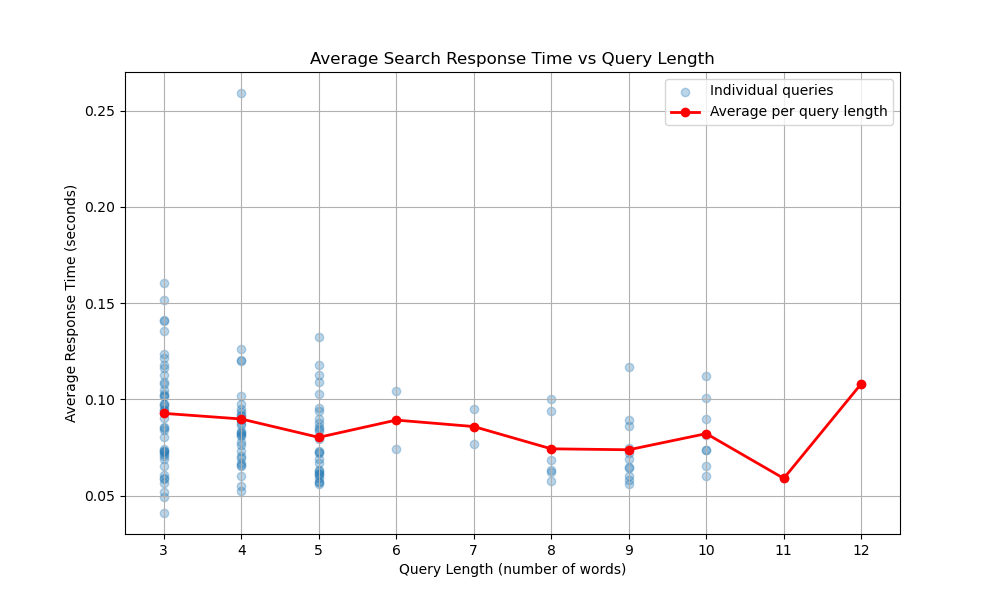
\includegraphics[height=.25\textheight]{res/avg_time_vs_query_length.png}
	\caption{Average response time vs.\ query length}
	\label{fig.response.time}
\end{figure}

\subsubsection{LLM invocation}
LLMs are invoked with two main purposes in the project, search query generation
from business topics, and filtering + synthesis of search results.

Table~\ref{tab.query.gen.result} lists the results of search query generation,
using inputs from LIST 1. They are collected from the output of
\texttt{llm\_\ttb pipeline.py}. The results demonstrate very high relevance to
the topic, although one of them cites an old year (\dots\ trends 2024
examples). A search query is judged as relevant, if it contains the exact
phrase or synonyms, or express the same meaning as the topic.
\begin{table}[hbtp!]
\centering
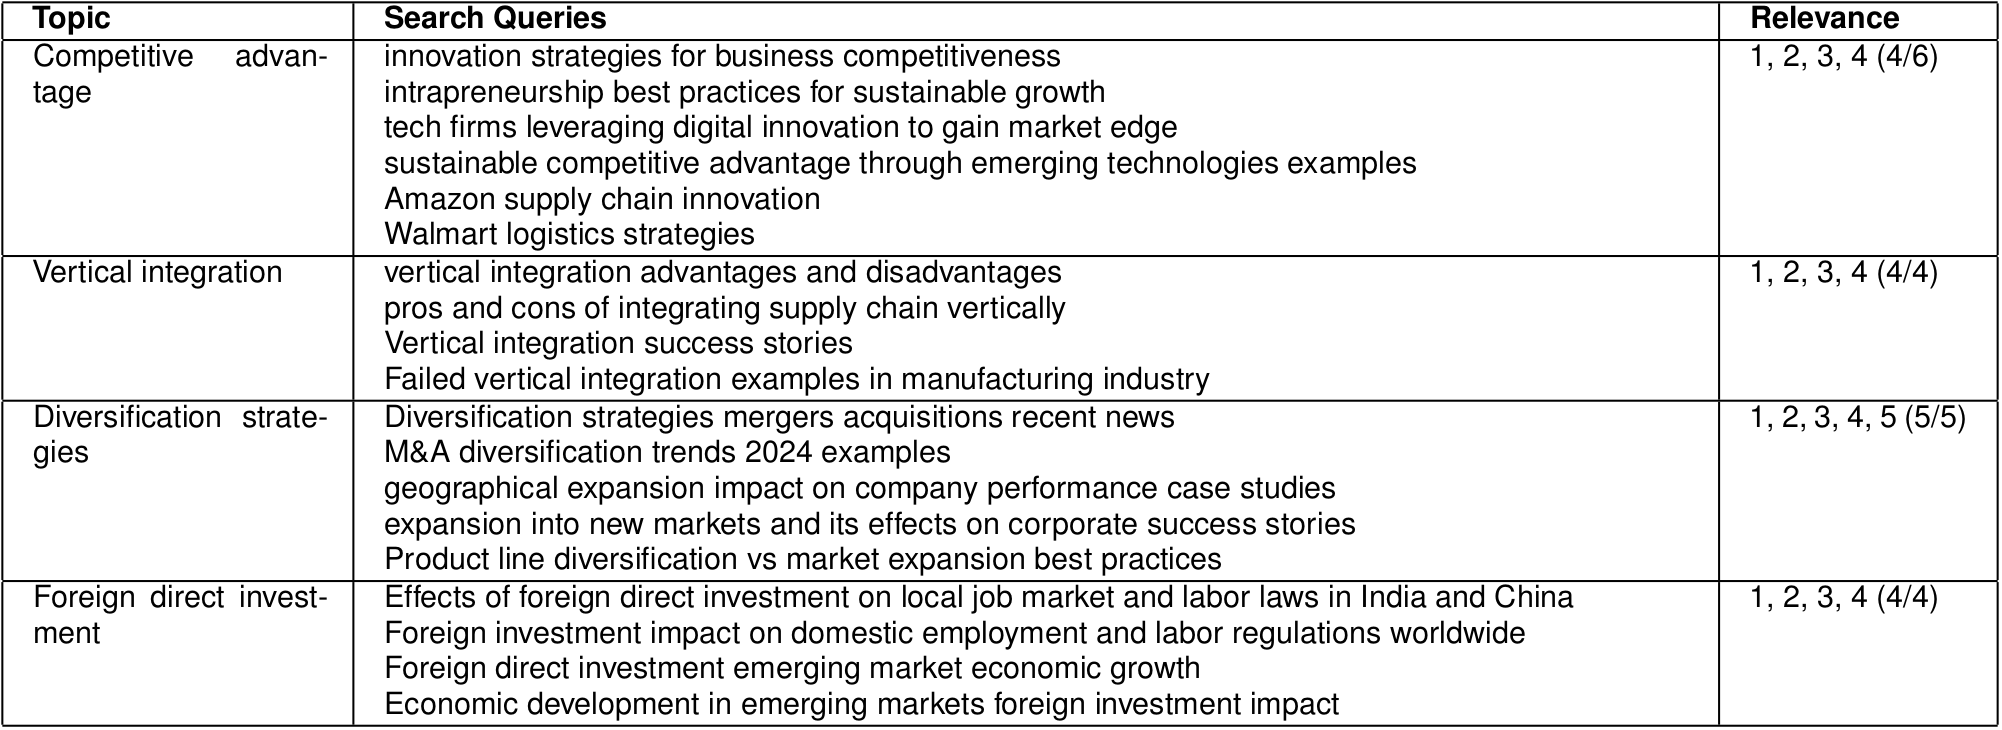
\includegraphics[width=.85\textwidth]{res/table_search_queries.png}
\caption{Relevance of generated queries}
\label{tab.query.gen.result}
\end{table}

The results of search summarization are even harder to qualify objectively. An
objective merit is that the LLMs can sometimes uncover surprising angles, while
an objective shortcoming is that the summarization quality sometimes cannot
meet expectation. One novalty in the summarization, only discovered in late
stage after several testing, is to make LLM output individually for each search
result a relevance number, which is used for filtering and reranking, instead
of giving all results to the LLM, in which case the LLM often distort the
search results.

\subsubsection{Walkthrough}
The full system starts with the user's configuring the system: business topics,
system prompts, automatic scheduelling, the accounts (sender email, destination
email, and Google search API key). All of them are configured on the GUI.

After the configuration, a setup script needs to be run to install the
schedualling tasks on the operating system. The user should also run the
indexer to initialize the custom search engine database. Then, at scheduled
times, the LLM pipeline and database updater will run.

The LLM pipeline starts by reading the business topics, then
\begin{enumerate}
	\item Invoke LLM to divide each topic into a diverse range of subtopics.
	\item Invoke LLM to generate search queries for each subtopic.
	\item Invoke both the custom search engine and Google's to produce search
		results and combine them.
	\item Invoke LLM to filter and rerank the search results.
	\item Invoke LLM to summarize all of them to a final report.
	\item Send the final report to the configured destination email addresses.
\end{enumerate}

The result includes both a final report and a directory of intermediate results
(e.g.\ search queries generated and raw search results), and thus cannot be
included in this word-count-limited thesis. Moreover, the use of LLM makes them
non-deterministic. The reader can instead run the pipeline herself to examine
output.

The database updater pulls the latest business news from the RSS feeds of
reputable Business sites, and then also removes the oldest documents from the
database, if the total number of documents exceeds a limit.

The user is free to reconfigure the system, and the changes will be reflected
the next time tasks are run.

\subsection{Results from mainstream tools}
I feed the same input to mainstream tools. Later in the Discussion section, I
will compare them with my system.

\subsubsection{ChatGPT}
When given the exact four topics used to produce
Table~\ref{tab.query.gen.result} and asked to summarize current business news
about them, GPT-4.1-mini produced remarkable result\footnote{
link \url{https://chatgpt.com/share/689a428d-f01c-8011-a115-57b4ca19a278}
}.
For each topic, it summarizes three recent examples that are all relevant.
However, from the sources it cites, a few issues can be identified:
\begin{enumerate}
	\item Some of the search results of ChatGPT did not originate from
		reputable Business news publishers, including sources from ``The Motley
		Fool'' and ``AInvest''.
	\item ChatGPT failed to find only sources from 2025, despite the presence of
		``current'' in the prompt.
\end{enumerate}

\subsubsection{Google}
The four topics are each separatedly given to the Google search engine, using
the phrase ``Current business news about [topic]''\footnote{Results as
	clickable links:
\href{https://www.google.com/search?q=Current+business+news+about+vertical+integration}{1}, 
\href{https://www.google.com/search?q=Current+business+news+about+diversification+strategies}{2}, 
\href{https://www.google.com/search?q=Current+business+news+about+competitive+advantage}{3}, 
\href{https://www.google.com/search?q=Current+business+news+about+foreign+direct+investment}{4}.
}.
Note that the results are purely identified by the URIs with the search queries
embedded in. As Google continues to update its service, there is no guarantee
that the observed results will remain the same.

Compared with ChatGPT, Google performed worse for all four topics. Each
results page contains some websites that describes/elaborates on the topic
itself or websites that act as a collection of articles on the topic, instead
of Business news about it. 

However, sometimes the AI Overview would trigger for the search results, but
that shares the same problems of ChatGPT. Worse than ChatGPT, Google's version
will also include webpages that are not news articles at all.
Figure~\ref{fig.results.google} displays Google's top results with and without
its AI Overview.
\begin{figure}[hbtp!]
	\centering
	
\includegraphics[width=.3\textwidth]{res/google_res1.png}
	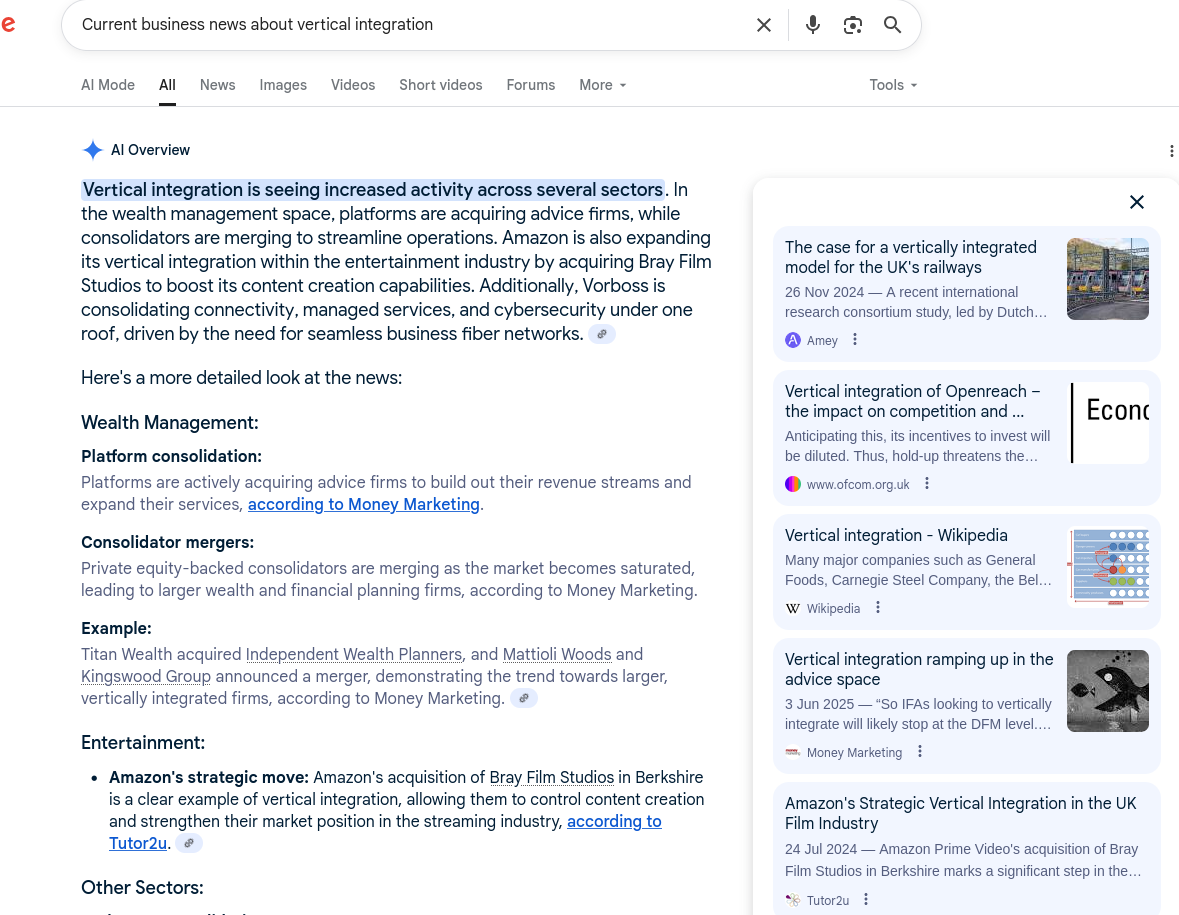
\includegraphics[width=.5\textwidth]{res/google_res2.png}
	\caption{Google results on the topics}
	\label{fig.results.google}
\end{figure}


\section{Discussion}
\subsection{Analysis of results}
\subsubsection{Alignment with design}
The system conforms to my design philosophy and methodology strictly, except
in a few places. 

Carefully designed OOP class hirerachy and interfaces are used in both C++
programs and Python scripts; interfaces of classes are chosen to make them
highly cohesive and loosely coupled. In C++, \texttt{const} is widely applied
to ensure immutability of data classes after construction. Comments cover all
functions, except for trivial ones whose name gives its meaning. Unit testing
were conducted for important features, because time constraints prevented me
to test all features. These together adhere to design philosophies 1--3.

Executables are separated to mostly doing one thing, often taking another's
output as input. This adheres to design philosophy 4.

Except for the optional feature of accepting user feedback and self-improving,
all features mentioned in methodology are implemented. 

\subsubsection{Fulfilment of goals}
Goal~1(a) is fulfilled, since the user only needs to give unstructured
text/images as input. One limitation of the system, however, is the lack of
support for other different file types, like lecture notes in PDF.

Goal~1(b) is fulfilled, by having a custom search engine only indexing
reputable Business news websites, and having both it and Google search only
results in specific date ranges. Both of the measures are deterministic,
providing reliability and accuracy to the system. Conversely, site-limiting
indexing inherently is inflexible and lack coverage of good information from
less reputable sources. A fixed range of dates also excludes the possibility to
include old discussions of concurrent events that spans a long time.

Goal~2 is fulfilled by the pipeline, which can be schedulled for execution,
once the user configured the system. Still, the automation can be further
improved by having a LLM generate all the configuration, with only a natural
language description from the user. Alternatively, I could exchange some
automation for more accuracy of the system, by having the pipeline interrupt
the user in the middle, asking her to select from the generated
subtopics/search queries.

Goal~3 is fulfilled by indexing only specific websites in the custom search
engine, too. Beside the inflexibility and coverage problem mentioned earlier,
the metric of reputability is inherently subjective. In this project, I took
advice from Sean O'Grady and consorted rankings of Business news
websites \cite{business.news.ranking.1, business.news.ranking.2}.

Goal~4 is fulfilled by using LLM only on real data from the search engines.
However, this cannot stop LLMs from hallucinating when generating search
queries or summarizing them.

The optional Goal~5 is not fulfilled.

\subsection{Comparsion with mainstream tools}
Against ChatGPT, my system successfully eliminated search results from
non-reputable sites. However, my system produced a few irrelavant search
queries and could not compete with ChatGPT in summary quality.

Versus Google, my system retrieved more reputable and current
information, but lacked in breadth. When Google's AI overview was triggered,
its summary quality also appeared to be superior.

Compared with the surveyed studies combining search engine of LLMs which have a
focus (either LLM4Search or Search4LLM) \cite{llm.meet.search.1}, my system is
a more neutral combination with a more general framework for information
retrieval. Orthognoal to their work aiming to address specific weakness of one
of the two, my work aims primarily to solve the specific information retrieval
problem.

\subsection{Examination by a real user}
Sean O'Grady, business school teacher, will be a real user of the
project. He examined carefully the result for the first item in LIST 1, and
informed me that 4 out of the 5 results would be useful to him and help him to
enhance the modules they are working on.

\subsection{Challenges and future plans}
The biggest engineering challenge overcome was implementing the custom search
engine. The indexing algorithm is simple, but a search engine spans
many different areas of computer science, networking, concurrency, program
design, database, algorithms. Many third-party libraries had to be picked and
used. Moreover, information retrieval on the current Internet is messy. One
particular problem was to handle different URL formats used by different
publishers.

The most significant optimization challenge was to fine-tune my pipeline and
LLMs. Tuning the prompts is complicated; changing a prompt to solve a current
problem may trigger another problem. The multi-stage design was consequently
implemented to ensure the LLM focuses on one problem at a time.

The system is significantly limited by the time-span of the project and my
resources. Particularly, I had no fund to purchase commercial LLM APIs and
could only rely on much less powerful local LLMs, constrained by local
computing resources. Additionally, the indexing database of my custom search
engine has to be built from scratch. Conversely, the minimal nature of my
system enables it to become a free personal solution running locally on PCs.

Most of the system's capabilities could be enhanced with more resources.
Nevertheless, there are a few design limitations to improve next: 
\begin{enumerate}
	\item Currently, the LLMs and search engines are loosely coupled (design
		philosophy 4). But in some cases integrating them more deeply (e.g.\ at
		the LLM model level) could be beneficial.
	\item Some parts are hard-coded to work for Business topics, damaging its
		potential to extend for general topics.
	\item The system is not designed to integrate with teaching platforms.
	\item The system is not designed to be cross-platform.
\end{enumerate}

\section{Conclusion}
I successfully designed a pipeline and developed a corresponding system
that combines LLMs with search engines to supply current content in business
school teaching. The system complements each individual tool substantially with
another, by limiting indexed websites, deterministic search results, and
multi-stage LLM invocation. Moreover, the system achieves more automation than
mainstream similar tools.

The methods worked considerably well in fulfilling my project goals.
Additionally, examination by a real user also proved its usefulness. However,
the system faces significant challenges to become a mature tool for general
public usage. While many of them could be mitigated by more resources, such as
purchasing a (more powerful) LLM API, or devoting more time to make it
cross-platform, the system's design choices exhibit some inflexibility, leaning
towards Business topics.

Although my system contributes as an engineering solution and an innovative
framework to integrate search engine and LLMs, it is not a theoretical
improvement of them; intrinsic problems like hallucination of LLMs and
non-semantical understanding of queries of search engines are still present.
Future work could also improve the two inherently and replace them in the
framework.

\clearpage

\bibliographystyle{plain} 
\bibliography{references.bib}

\end{document}          
